\section{Dynamical variables}
Dynamical variables are aset of variables that describe a system that changes
over time. Equations of motion describe how these variables change. With
Newtonian physics we relied on knowing about precise initial conditions before
we had a clue what was going on.

\section{Degrees of Freedom} 
Point masses have three degrees of freedom, in the $x$, $y$, $z$ planes. A
system of $M$ point masses have:
$$	
	N = 3M
$$
degrees of freedom (3 for each particle). However, the existence of $j$
independent constraints (rigid `bars' between the masses) reduces this to:
$$
	N = 3M - j
$$
This leads to the conclusion that any rigid body with more than two point masses
connected with rigid rods has exactly 6 degrees of freedom - $x$, $y$, $z$ of
the centre of mass, along with three angles to describe the orientation. Another
way of specifying this is simply to give two points within the plane.

\subsection{Constraints and their types}
The existance of these $j$ constraints means that the masses, $M$, are no longer
independent. To describe the system fully (as long as we know what the system
looks like), we only need as many co-ordinates as there are degrees of freedom.

If the constraints are \emph{holonomic} then it is possible to express the
full position and orientation of the system, $\bm{r}$ as a function of these
co-ordinates $q_k$:
$$
	\bm{r} = \bm{r}(q_1, q_2, \hdots, q_N, t).
$$
There are two types of holonomic constraints:
\begin{itemize}
	\item Rheonomic - time dependent constraint
	\item Scleronomous - no \emph{explicit} time dependence
\end{itemize}
If we can express the constraints as a function:
$$
    \bm{r} = \bm{r}(q_1, q_2, \hdots, q_N, t) = 0,
$$
Then they are all holonomic.

Constraints are non-holonomic if the state depends on the path taken to achieve
it - differential constraints or inequalities. These are usually velocities.

\subsection{Examples}
\paragraph{Example 1:} point mass on an inclined plane.
\begin{figure}[h!]
	\centering
	\includegraphics[width=0.5\textwidth]{PointMassOnInclinedPlane.png}
\end{figure}
Here, we can find that all constraints are holonomic if we say:
$$
	\tan\theta = \frac{x}{z} ;\ \rightarrow \;
	z\tan\theta - x = 0
$$
This describes the system fully.

\paragraph{Example 2:} bead on a rotating wire.
\begin{figure}[h!]
    \centering
	\includegraphics[width=0.5\textwidth]{BeadOnRotatingWire.png}
\end{figure}
For the rotating wire, we find two equations that both have time dependence and
hence are \emph{rheonomic}:
$$
	x = z\tan\theta\cos\omega t
$$
$$
	y = z\tan\theta\sin\omega t
$$
These constraints mean that the particle always lies on the wire.

\paragraph{Example 3:} coin, rolling on a plane.
\begin{figure}[h!]
	\centering
	\includegraphics[width=0.5\textwidth]{CoinOnPlane.png}
\end{figure}
This is slightly more complicated, and is also non-holonomic:
$$
	\mathrm{d}x = a\mathrm{d}\theta \cos \phi
$$
$$
	\mathrm{d}x = a\mathrm{d}\theta \sin \phi
$$
If we say that the angle that the coin has turned is $\theta$. We can reach any
point in this 4D space - i.e. we cannot separate the constraints from the
dynamics.

